


\section{Energy Sensors}


In this section is covered the theory behind energy sensors as well as the technologies used. In subsection \ref{subs:321} is started the presentation of the electric energy. Further on, in subsection \ref{subs:322} is covered the energy transducers and in subsection \ref{subs:323} is presented the challenges and requirements of energy measurement in \ac{RTS}. 
%This section is concluded with the presentation of the technologies used in RTS for energy measurement purposes.

\subsection{Electric Energy Overview}
\label{subs:321}
Energy in form of electricity is the major traction player on the \ac{RTS}. 
Complementary to the Diesel, this form of energy is distributed along with the rails in catenaries.
As presented in previous section, there are two major ways of rail electrification: \ac{AC} or \ac{DC}.

When a train is connected to a DC transmission line, it is possible to exchange energy from and to the catenary, complying to the Kirchhoff's circuit laws. The catenary is considered as a node that has multiple bi-directional power flow elements, specifically, trains and traction substations.

On \ac{AC} transmission lines, the power flow is directly related to the relation between the voltage and current waveforms, as presented in figures \ref{fig:traction} and \ref{fig:generation}.

\begin{figure}[h!]
	\centering
	\begin{minipage}{.48\textwidth}
		\centering
		%		\vspace{2.5em}
			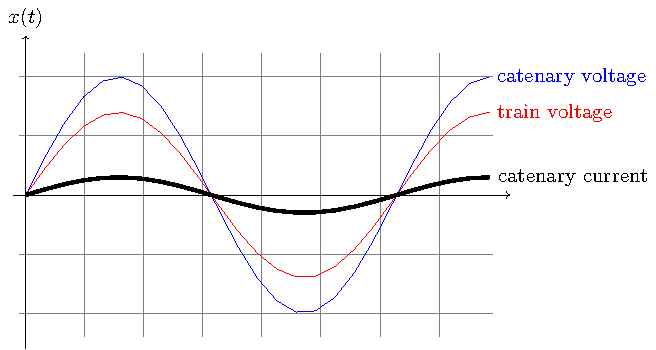
\includegraphics[width=1\textwidth,keepaspectratio]{figures/32.EnergyS/traction}
		%		\vspace{2em}
		\captionof{figure}{Waveforms in traction mode.}
		\label{fig:traction}
	\end{minipage}%
	\begin{minipage}{.01\textwidth}  ~\end{minipage}	
	\begin{minipage}{.48\textwidth}
		\centering
		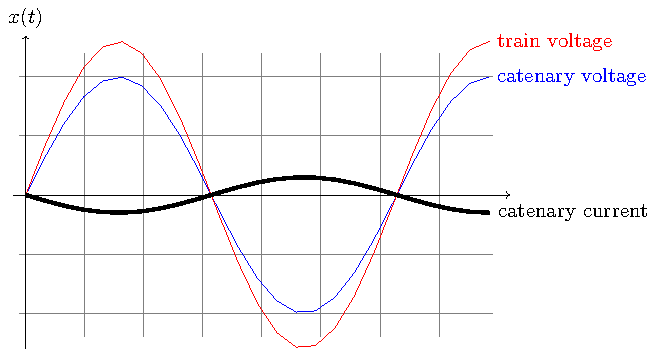
\includegraphics[width=1\textwidth,keepaspectratio]{figures/32.EnergyS/generation}

		
		%		\vspace{0.5em}
		\captionof{figure}{Waveforms in generation mode.}
		\label{fig:generation}
	\end{minipage}
\end{figure}

The energy calculation depends on the voltage and currents measured in the catenary. This function present in train energy meters evaluates the voltage and currents and generates the active, reactive and power factor information of the train. In figure \ref{fig:liran2014} is presented an example of the energy information 1h operation of {$HX_D1B$} locomotive.


\begin{figure}[h!]
	\centering
	\begin{minipage}{0.9\textwidth}
		\centering
				\vspace{-0.75em}
		\includegraphics[width=0.65\textwidth,keepaspectratio]{figures/32.EnergyS/liran2014}
				\vspace{-0.75em}
		\captionof{figure}{1h waveforms of active power (black), reactive power (red) and power factor (blue) of {$HX_D1B$} locomotive.  Adapted from \cite{liran2014}.}
		\label{fig:liran2014}
	\end{minipage}%
	
\end{figure}


\subsection{Current transducers and voltage transducers}
\label{subs:322}	
	According to Pallàs-Areny and Webster (2012), a transducer is a device capable to convert different physical signal forms, \cite{webster2012}. In the scope of energy measurements, current and voltage transducers are employed. These devices convert the field energy waveforms into a voltage (or current) waveform capable of be acquired by a processing unit (such as a microcontroller, programmable logic controller, etc.).
	
	Dalessandro et al. (2007) identifies multiple different physical effects associated to the current sensors %\footnote{In the scope of energy measurements, voltage transducers combine the measurement of a current in a given load (or resistor). Therefore this subsection will only cover the measurement of currents} 
	as following, \cite{Dalessandro2007}:
	
	\begin{description}
		\setlength\itemsep{-0em}
		\item [Magnetic coupling] Using the knowledge of transformers, it is possible to perform isolated current measurements. The current transformers are widely used in energy measurement and are based on the magnetic coupling concept, with a ferromagnetic core. With the same magnetic coupling principle, the Rogowski coil is a helix wound around a non-magnetic torus and uses the magnetic coupling physical effect to measure the current, as the integrative of the induced voltage on coil terminals;
		%5-7
		\item [Magneto resistance] The anisotropic magneto-resistive current sensors uses a magneto-resistive sensing element (composed of a nickel iron alloy) to measure the magnetic field induced by a current on a conductor;
		%8,9
		\item [Faraday induction] Fiber optic current sensors relies on Faraday effect to integrate the magnetic field along the closest path. The magnetic field will cause a magnetooptic phase shift of the light waves and this phase shift is measured with a technique known as fiber gyroscopes;
		%10
		\item [Hall Effect] Similarly to magneto-resistive current sensors, the hall effect sensors uses a sensing element to measure the magnetic field in the air-gap of a magnetic circuit. For AC-only current measurement, no compensation of the flux in the magnetic core is made. The implementation of "Zero flux" compensation avoids the saturation of the magnetic core. This active compensation allows the measurement of currents with DC component.
		
	\end{description}

	The voltage transducers depend of an indirect measurement of the electric field. In particular, the principle is the combination of the current measurement in a known load (or resistor), connected to the terminals of the circuit intended to be measured and using the principles previously presented. In figures \ref{fig:current_t} and \ref{fig:voltage_t} are presented two transducers used for energy measurement in RTS.
	
	\begin{figure}[h!]
		\centering
		\begin{minipage}{0.45\textwidth}
			\centering
			%		\vspace{2.5em}
			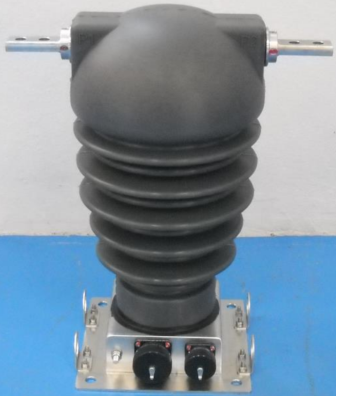
\includegraphics[width=0.32\textwidth,keepaspectratio]{figures/32.EnergyS/current_t}
			%		\vspace{2em}
			\captionof{figure}{25 kV current transformer. Adapted from www.railware.it}%\footnotetext{www.railware.it}}
			\label{fig:current_t}
		\end{minipage}%
		\begin{minipage}{0.05\textwidth}  ~\end{minipage}	
		\begin{minipage}{0.45\textwidth}
			\centering
			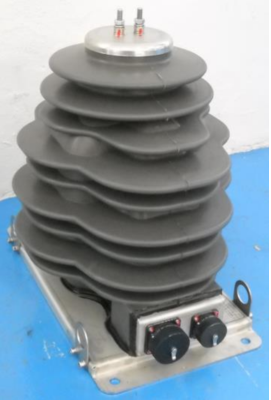
\includegraphics[width=0.25\textwidth,keepaspectratio]{figures/32.EnergyS/voltage_t}
			
			
			%		\vspace{0.5em}
			\captionof{figure}{25 kV voltage transformer. Adapted from www.railware.it}%\footnotetext{www.railware.it}}
			\label{fig:voltage_t}
		\end{minipage}
	\end{figure}
	
%\vspace{-2em}
\subsection{Energy measurement in RTS}	
\label{subs:323}

	Currently, the European Commission requires the implementation of mechanisms in \ac{RTS} for energy liberalization, where the \ac{RUs} can purchase energy from suppliers of their choice, \cite{eur-lex2008}.
	
	The impact of such requirement is the liberalization of the energy market, which brings new challenges in the railway sector. In practical, on-board energy metering is important to make energy savings visible and to allocate the profits of these savings to the respective RUs.
	
	As an example, EcoS energy meter for railway, presented in figure \ref{fig:ecos}, identifies the following requirements to comply with:
	
	\begin{description}
	\setlength\itemsep{-0em}
	
	\item [EN 50463 standard \cite{EN50463}] This standard defines the architecture of the Energy Measurement System. It is composed by two blocks: (1) the Energy Measurement Function, responsible for the measurement of voltage and current and for the calculation of the energy and (2) the Data Handling System, that joins the timestamp and the GPS location to the energy data. In section \textit{3.4: Smart Metering}, the components of this standard are better described;
	
	\item [EN 50155 standard \cite{EN50155}] This standard defines the aspects of temperature, humidity, shock, vibration, and other parameters that covers electronic equipment used on rolling stock for railway applications;
	
	\item [\ac{AC} and \ac{DC} measurement channels] The energy meter comply with multiple catenary topologies;
	
	\item [Multiple Connectivity] EcoS uses WiFi, Ethernet and 2G/3G/4G. In addiction it is used the localization and time sync from \ac{GPS} and \ac{TCMS};
	
	\item [Multiple access and customization] EcoS implements web interface and a SoftPLC for expansions and customizations.
	\end{description}



\begin{figure}[h!]
	\centering
	\begin{minipage}{.8\textwidth}
		\centering
		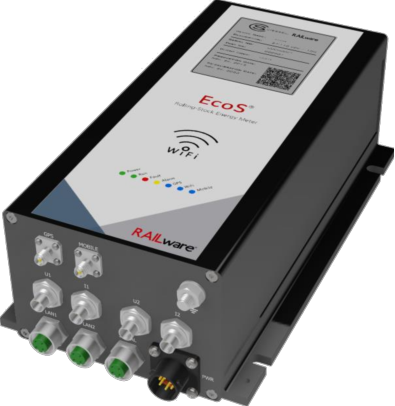
\includegraphics[width=0.35\textwidth,keepaspectratio]{figures/32.EnergyS/ecos}
		%		\vspace{0.5em}
		\captionof{figure}{EcoS railway energy meter. Adapted from railware.it}
		\label{fig:ecos}
	\end{minipage}
\end{figure}

	\newpage
	
\subsection{Energy measurement function}
\label{subs:324}

With the compliment of the EN50463 standard, the EcoS energy meter performs the energy calculations as presented in figure \ref{fig:energy_calculation}.

\begin{figure}[h!]
	\centering
	\begin{minipage}{.8\textwidth}
		\centering
		\vspace{-0.5em}
		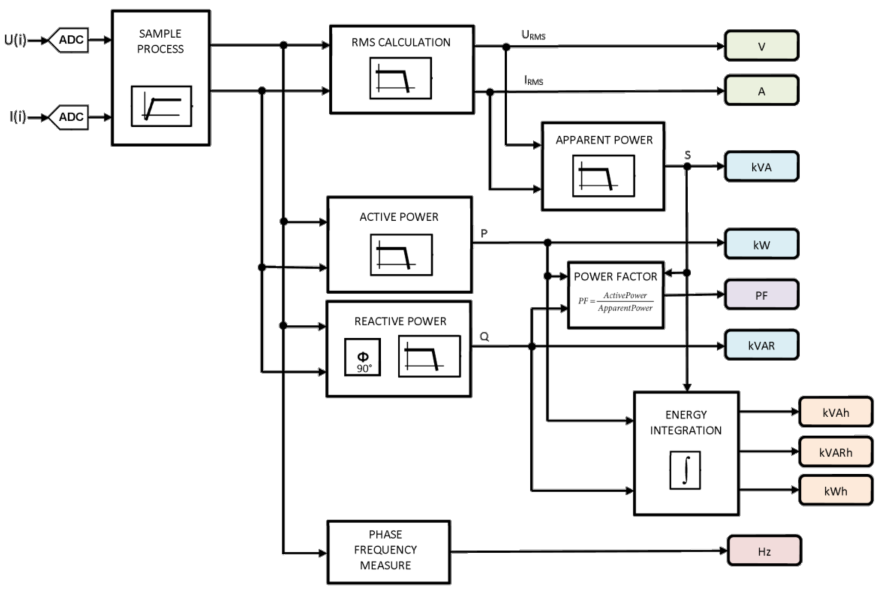
\includegraphics[width=\textwidth,keepaspectratio]{figures/32.EnergyS/energy_calculation}
		%		\vspace{0.5em}
		\captionof{figure}{EcoS power calculation function. Adapted from railware.it}
		\label{fig:energy_calculation}
				\vspace{-1em}
	\end{minipage}
\end{figure}

\begin{comment}


\subsection{Energy measurement technologies in RTS }
\label{subs:324}



\begin{figure}[h!]
	\centering
	\begin{minipage}{0.40\textwidth}
		\centering
		%		\vspace{2.5em}
		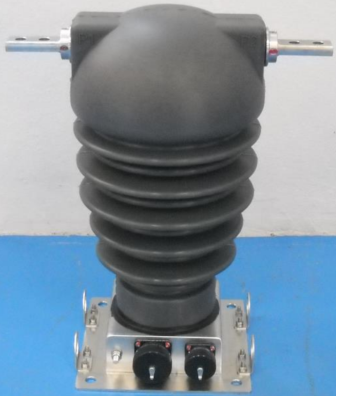
\includegraphics[width=0.75\textwidth,keepaspectratio]{figures/32.EnergyS/current_t}
		%		\vspace{2em}
		\captionof{figure}{25 kV current transformer. Adapted from ?}%\footnotetext{www.railware.it}}
		\label{fig:current_t}
	\end{minipage}%
	\begin{minipage}{0.05\textwidth}  ~\end{minipage}	
	\begin{minipage}{0.40\textwidth}
		\centering
		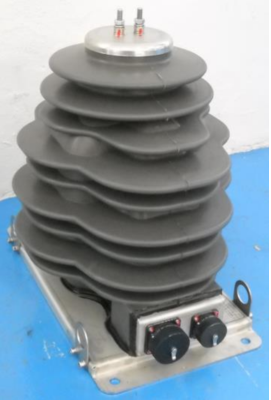
\includegraphics[width=0.59625\textwidth,keepaspectratio]{figures/32.EnergyS/voltage_t}
		
		
		%		\vspace{0.5em}
		\captionof{figure}{25 kV voltage transformer. Adapted from ?}%\footnotetext{www.railware.it}}
		\label{fig:voltage_t}
	\end{minipage}
\end{figure}

\end{comment}


